\chapter{Solving the challenge}

In order to solve the challenge you will only need:
\begin{itemize}
	\item{Understanding how integer overflows and truncation work in memory (at bit level).}
	\item{A calculator with bit-view mode, and preferably bit-toggling capabilities, in order to help you visualize what is actually happening. Windows10's default calculator in Programmer is awesome. As a Linux alternative you can use KCalc\footnote{\url{https://kde.org/applications/utilities/org.kde.kcalc}}.}
\end{itemize}

\begin{figure}[h]
	\makebox[\textwidth][c]{
		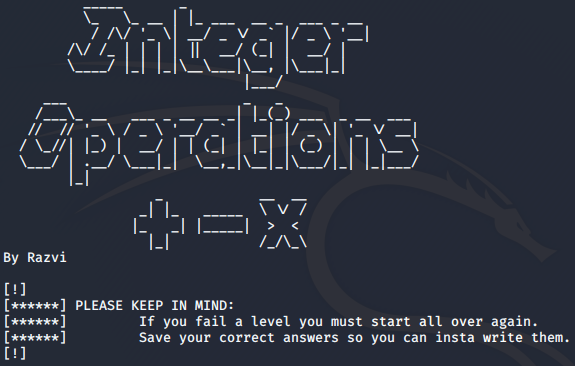
\includegraphics{binary_intro.png}
	}
	\label{fig:binary_intro}
	\caption{Binary's introduction.}
\end{figure}

%%%%%%%%%%%%%%%%%%%%%%%%%%%%%%%%%%%%%%%%%%%%%%%%%%%%%%%%%%%
\section{Level 1: Basics of addition}

\begin{figure}[h!]
	\makebox[\textwidth][c]{
		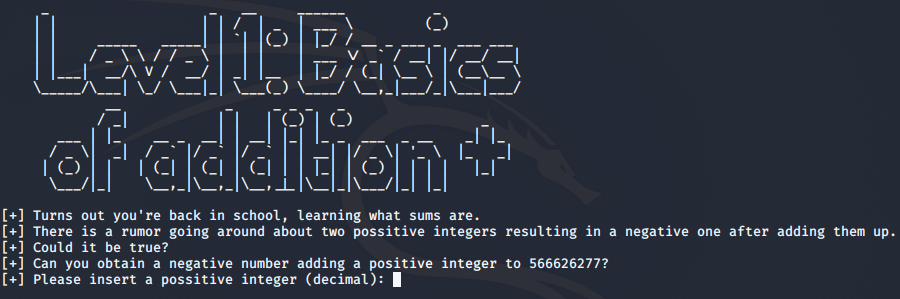
\includegraphics[scale=.8]{intro_level1.png}
	}
	\label{fig:intro_level1}
	\caption{Formulation of the first level.}
\end{figure}

\begin{figure}[h!]
	\makebox[\textwidth][c]{
		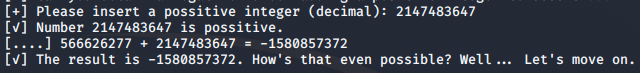
\includegraphics[scale=1]{solved_level1.png}
	}
	\label{fig:solved_level1}
	\caption{Solving the first level.}
\end{figure}

%%%%%%%%%%%%%%%%%%%%%%%%%%%%%%%%%%%%%%%%%%%%%%%%%%%%%%%%%%%%s
\section{Level 2: Basics of subtraction}

\begin{figure}[h!]
	\makebox[\textwidth][c]{
		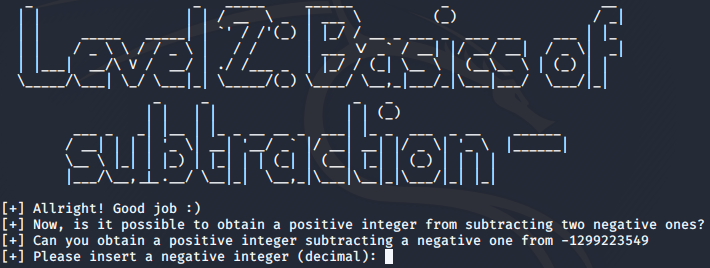
\includegraphics{intro_level2.png}
	}
	\label{fig:intro_level2}
	\caption{Formulation of the second level.}
\end{figure}

\begin{figure}[h!]
	\makebox[\textwidth][c]{
		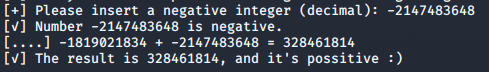
\includegraphics[scale=1]{solved_level2.png}
	}
	\label{fig:solved_level2}
	\caption{Solving the second level.}
\end{figure}

%%%%%%%%%%%%%%%%%%%%%%%%%%%%%%%%%%%%%%%%%%%%%%%%%%%%%%%%%%%%%%
\section{Level 3: Simple equations}

\begin{figure}[h!]
	\makebox[\textwidth][c]{
		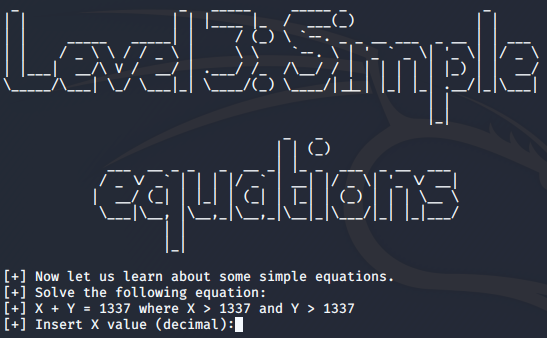
\includegraphics{intro_level3.png}
	}
	\label{fig:intro_level3}
	\caption{Formulation of the third level.}
\end{figure}

\begin{figure}[h!]
	\makebox[\textwidth][c]{
		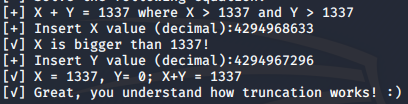
\includegraphics[scale=1]{solved_level3.png}
	}
	\label{fig:solved_level3}
	\caption{Solving the third level.}
\end{figure}

%%%%%%%%%%%%%%%%%%%%%%%%%%%%%%%%%%%%%%%%%%%%%%%%%%%%%%%%%%

\section{Level 4: Twisting the numbers}

\begin{figure}[h!]
	\makebox[\textwidth][c]{
		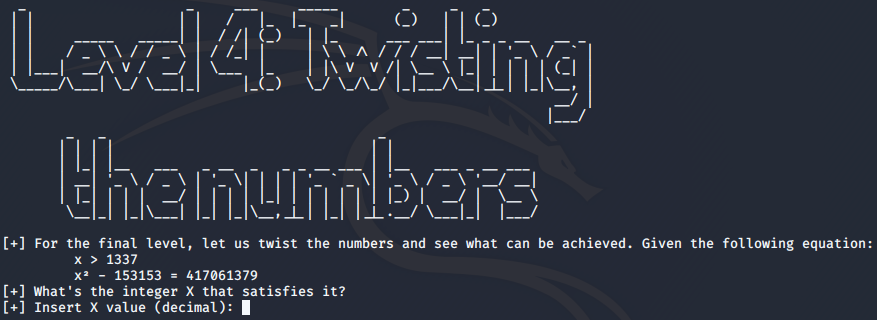
\includegraphics{intro_level4.png}
	}
	\label{fig:intro_level4}
	\caption{Formulation of the forth and last level.}
\end{figure}

\begin{figure}[h!]
	\makebox[\textwidth][c]{
		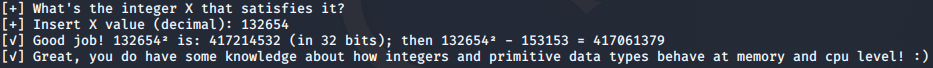
\includegraphics[scale=1]{solved_level4.png}
	}
	\label{fig:solved_level4}
	\caption{Solving the forth and last level.}
\end{figure}